
\section{MOEA/D}\label{sec:background} 

\begin{figure*}[!t]\label{decomp-example}
	\centering
	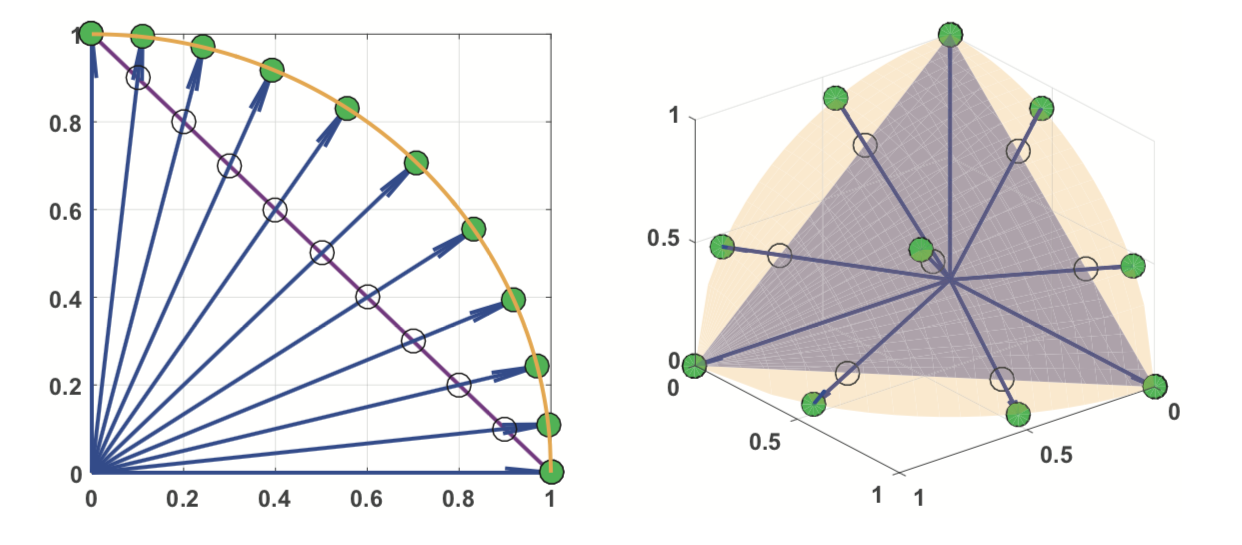
\includegraphics[width=\textwidth]{images/decomp2.png}
	\caption{Decomposition  -  2 and 3 objectives - Figure from \cite{chugh2017handling} }
\end{figure*}.

Here, MOEA/D~\cite{zhang2007moea} is briefly explained. MOEA/D represents a class of population-based meta-heuristics for solving Multi Objective Problems (MOPs). It is based on decomposition, which is one kind of scalarizing function, where one multi-objective problem becomes various single-objective sub-problem. That is, MOEA/D decomposes an MOP with $n_f$ objectives, as defined in equation~\ref{min_problem}, into $N$  sub-problems using a set of uniformly distributed weight vectors. To define the sub-problem a weight vector is used as a decomposition strategy to  define the sub-problems.  All these $N$ sub-problems are expected to represent a good approximation to the PF, as it is shown in Figure~\ref{decomp-example}.

MOEA/D solves these subproblems simultaneously by evolving a set of solutions in a single run by using a aggregation function. This function allied with the weight vectors need to guarantee that a optimal solution to a sub-problem is Pareto-optimal for the MOP and also need to guarantee that the solutions are well distributed in the space of objectives. Therefore, the set of solutions may provide a fair approximation of the Pareto Front.

The relationship between the set of solutions and the sub-problems is formulated as for every sub-problem a unique solution is associated to it, thus the size of the set of solutions is equal to the number of sub-problems.  At each interaction, one new candidate solution is generated by applying a sequence of variation operators to the existing solutions. This new solution is then compared with the old one, and the best solution after is maintained as the incumbent solution given the procedure defined by the update strategy.

To compare the solutions or to generate a new one, the algorithm utilizes a neighborhood that defines the limits the exchange of information of a sub-problem between candidates solutions. This neighborhood is defined based on the distance among their weights.



\IncMargin{1em}
\begin{algorithm}
\LinesNumbered
	\KwIn{Objective functions \textbf{f}; constraint functions \textbf{g}; input parameters}
	t$\rightarrow$ 0\\
	\textit{run} $\rightarrow$ TRUE\\
	Initialize the solution set $ X^{(t)} =  {x^1, ..., x^{n_{f}}}$ by random sampling from $\Omega$
	Generate weights $\Lambda$\\
	%
	%\For{$i \in {1,...,n_f}$}{Set the neighborhood index list $B^i = {1_i, ..., i_T}$;}
	%
	%
	\While{run}{
		Define or update neighborhood $B^i = {1_i, ..., i_{n_{f}} } $\\
		Copy incumbent solution set $X'^{(t)}$ into $X'^{(t)} $\\
		\For{each variation operator $v \in V$}{
			$X^{(t)} \leftarrow v(X'^{(t)})$
		}
	Evaluate solutions in $X^{(t)}$ and $X'^{(t)} $
	
	Define next population $X^{(t+1)}$
	Update \textit{run}  flag
	t$\rightarrow$ t + 1
	}
	\textbf{return} 	$X^{(t)}$, f$(X^{(t)})$
	%		
	%		
	\caption{General procedure of MOEA/D framework}
\end{algorithm}\DecMargin{1em}


